\subsection{Nutzeranforderungen und Systemanforderungen}
\label{sec:Kap-6.2.1}

Abbildung~\ref{fig:nutzer-vs-system} zeigt die Einteilung von Anforderungen in Nutzeranforderungen, System\-anforderungen und domänenbasierte Anforderungen. Hierbei handelt es sich um eine Kategorisierung anhand unterschiedlicher Blickwinkel. Nutzeranforderungen fokussieren den Blickwinkel "`Was möchten Nutzer (und Auftraggeber) tun bzw. vorfinden?"'. Systemanforderungen beschreiben "`Was muss das System dafür können bzw. gewährleisten?"'. Und domänenbasierte Anforderungen berücksichtigen die Ebene "`Welche (zusätzlichen) Anforderungen liefert die Domäne?"'.

\vspace{\baselineskip} %%% für Druck
\vspace{\baselineskip} %%% für Druck

\begin{figure}[h!]
	\centering
	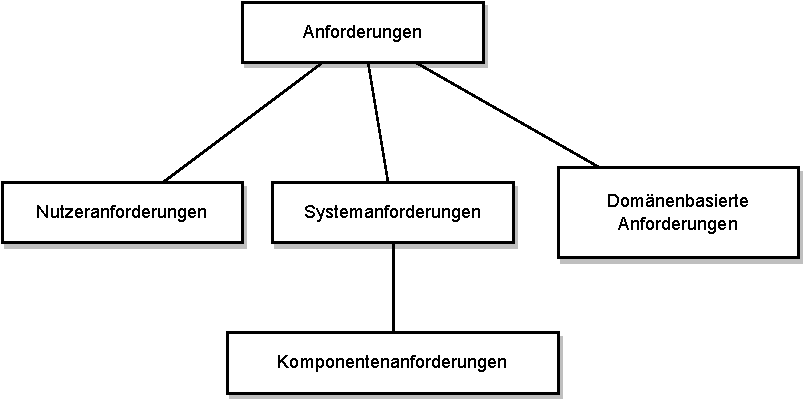
\includegraphics{Bilder/Kapitel-6/nutzer_vs_system.pdf}
	\caption{Nutzer-, System- und domänenbasierte Anforderungen}
	\label{fig:nutzer-vs-system}
\end{figure}

\vspace{\baselineskip} %%% für Druck

\minisec{Nutzeranforderungen}

Nutzeranforderungen sind Anforderungen, die aus Sicht und in der (Domänen)
\linebreak %%% für Druck
Sprache der Kunden formuliert sind. Sie sind die Form, in der Kunden ihre Bedürfnisse kommunizieren. Den größten Anteil an den Nutzeranforderungen haben Anforderungen, die das extern sichtbare Verhalten des Softwaresystems betreffen. Sie beschreiben, was ein Nutzer mit der Software tun will: welche Aktionen er ausführen können möchte und welche Ergebnisse er dabei erwartet. Aber auch Anforderungen, die das äußere Erscheinungsbild des Softwareprodukts betreffen (wie die Berücksichtigung des Coporate Design des Auftraggeber-Unternehmens oder die Gestaltung von Benutzeroberflächen), Anforderungen des Kunden an Qualitätsmerkmale des Produkts (\zb einfache Bedienbarkeit, schnelle Erlernbarkeit, das Vorhandensein kontextsensitiver Hilfe etc.) oder Kundenwünsche nach Schnittstellen zu Hard- und Softwaresystemen des Systemkontexts gehören zu den Nutzeranforderungen. Nutzeranforderungen sollten immer von einem zu erreichenden Ziel bzw. einem zu lösenden Problem der Stakeholder ausgehen: Eine Anforderung, für die selbst der Anforderungssteller nicht begründen kann, welchen Zweck sie erfüllt, wird in der Regel zu nicht genutzten Funktionalitäten oder unnötigen Eigenschaften des Softwareprodukts führen und dabei Entwicklungsressourcen verschwenden.

\vspace{2mm} %%% für Druck

\sttpseitenrandzitat{"`If your software does not have to satisfy a need, then you can build anything. However, if it is meant to satisfy a need, then you have to know what need is to build the right software"'}{\cite[3]{rob13}}

\vspace{2mm} %%% für Druck


Nutzeranforderungen können unterschiedlich stark ausdifferenziert sein. Eine recht abstrakte Nutzeranforderung auf einer hohen Ebene aus dem Zookontext könnte lauten:

\vspace{2mm} %%% für Druck

\sttpAnforderungText{Potentielle Zoobesucher sollen im Internet über neugeborene Tiere informiert werden.}

\vspace{\baselineskip} %%% für Druck

Ein zu erreichendes Ziel hinter dieser Anforderung könnte -- unter der Annahme, dass Babytiere Besuchermagneten sind -- die Erhöhung des Besucheraufkommens des Zoos sein. Die Anforderung ist aber so allgemein gehalten, dass man nicht bestimmen kann, welche Funktionalität der zukünftigen Software der Anforderungssteller genau einfordert. Eine detailliertere Nutzeranforderung aus dem gleichen 
\linebreak %%% für Druck
Kontext wäre:

\vspace{2mm} %%% für Druck

\sttpAnforderungText{Tierpfleger sollen die Namen neugeborener Tiere angeben können, um diese auf der Zoo-Website anzeigen zu können.}

\vspace{\baselineskip} %%% für Druck

Oder als sogenannte User Story formuliert, wie es vor allem in agilen Entwicklungsprojekten praktiziert wird:

\vspace{2mm} %%% für Druck

\sttpAnforderungText{Als Tierpfleger möchte ich den Namen eines neugeborenen Tiers angeben können, um diesen auf der Zoo-Website anzeigen zu lassen.}

\pagebreak %%% für Druck

\minisec{Systemanforderungen}

Aus einer solchen Nutzeranforderung ergeben sich Anforderungen an die Dienste des zukünftigen Softwareprodukts. Also: welche Bedingungen muss die Software \mbox{gewährleisten} bzw. welche Fähigkeiten muss sie besitzen, um die Nutzeranforderung erfüllen zu können. Im Beispiel muss sie die Möglichkeit bieten, die Namen der Tiere (irgendwie) zu erfassen, sie speichern, auf die gespeicherten Informationen zugreifen können und diese anzeigen können. Eine entsprechende Anforderung könnte lauten:

\vspace{2mm} %%% für Druck

\sttpAnforderungText{Die Software soll die Namen neugeborener Tiere erfassen, speichern und anzeigen.}

\vspace{\baselineskip} %%% für Druck

Eine solche, durch Verfeinerung einer Nutzeranforderung entstandene Anforderung nennt man eine Systemanforderung. Systemanforderungen beschreiben, welche
\linebreak %%% für Druck
Eigenschaften und Funktionalitäten die zukünftige Software aufweisen soll, um die in den Nutzeranforderungen ausgedrückten Bedürfnisse der Nutzer umsetzen zu können. Sie werden auf Grundlage der Nutzeranforderungen in Zusammenarbeit zwischen Kunden und Softwareentwicklungsteam erstellt. Wie Nutzeranforderungen können Systemanforderungen einen unterschiedlichen Detaillierungsgrad aufweisen. Die Systemanforderung könnte in einer konkreteren Form auch lauten:

\vspace{2mm} %%% für Druck

\sttpAnforderungText{Die Namen neugeborener Tiere sollen über Eingabemasken erfasst, in einer Datenbank gespeichert und als Liste angezeigt werden.}

\vspace{\baselineskip} %%% für Druck

Systemanforderungen sind weiterhin Anforderungen und keine Entwurfsbeschreibungen, welche erläutern, in welcher Weise Anforderungen im Softwaresystem umgesetzt werden. Dementsprechend sollten sie noch weitgehend lösungsneutral formuliert werden. Ähnlich wie bei den Zielen (Kap.~\ref{sec:Kap-6.1.2.2}) können aber Nutzer\-bedürfnisse oder Rahmenbedingungen bestehen, die den möglichen Lösungsraum einschränken. So sollte im Beispiel von oben die Erfassung der Tiernamen über Eingabemasken durchaus schon in der Anforderung thematisiert werden, wenn für den Kunden keine andere Art der Erfassung (\zb über das Hochladen von strukturierten Daten oder Dateien) in Frage kommt. Insgesamt ist die Grenze zwischen System\-anforderungen und Systembeschreibung fließend. Gerade bei sehr detailliert ausgearbeiteten Systemanforderungen ist man nicht mehr weit von einer Umsetzungs\-beschreibung entfernt. Der folgende Kasten zeigt an einem Beispiel den Unterschied zwischen einer Nutzeranforderung und einer Systemanforderung und vermittelt \mbox{Ihnen} zudem einen Eindruck von dem Unterschied zwischen Systemanforderung und Umsetzungsbeschreibung.

\pagebreak %%% für Druck

\sttpKasten{\textbf{Beispiel}
\\
\\
\underline{Nutzeranforderung:} Das System muss dem externen Abrechnungssystem der Tierärzte die notwendigen Informationen über die Behandlung der Zootiere zur Verfügung stellen können.
\\
\\
\underline{Systemanforderung:} Es muss eine Schnittstelle zwischen dem neuen Zooverwaltungssystem und dem von der Tierärztlichen Abrechnungsstelle betriebenen Abrechnungssystem eingerichtet werden. Über diese Schnittstelle müssen für jede Zootierbehandlung spätestens 2~Werktage nach der Behandlung folgende Informationen an das Abrechnungssystem übergeben werden: Name und Identifikationsnummer des Tierarztes, Identifikationsnummer des Zoos, \mbox{Name} und Art des Tiers, Art und Dauer der Behandlung, eingesetzte Medikamente.
\\
\\
\underline{Umsetzungsbeschreibung:} Das externe Abrechnungssystem bietet eine spezielle Webschnittstelle für Zoos an, über die Informationen in einem vorgegebenen JSON\footnote{JSON: JavaScript Object Notation. Ein Dateiformat in einer menschlich lesbaren Textform, welches zum Datenaustausch zwischen verschiedenen Anwendungen verwendet wird, s. \url{https://de.wikipedia.org/wiki/JavaScript_Object_Notation}}-Format an das Abrechnungssystem übertragen werden können. Das Zooverwaltungssystem wird diese Webschnittstelle nutzen, die in beiliegender Tabelle spezifizierten Informationen entsprechend ihres jeweiligen Datentyps in die benötigten Einträge des JSON-Formats transformieren und alle 48~Stunden automatisiert die jeweils neuen Datensätze übertragen. 
}

Eine \marginline{Kom\-po\-nen\-ten\-an\-for\-de\-run\-gen} eigene Unterkategorie von Systemanforderungen bilden die sogenannten Komponentenanforderungen. Diese legen den Blickwinkel auf eine konkrete Komponente des zukünftigen Systems und beschreiben, welchen Beitrag diese Komponente für bestimmte Systemanforderungen leisten soll. Die explizite Formulierung von Komponentenanforderungen spielt vor allem dann eine Rolle, wenn für ein zu entwickelndes Softwareprodukt vorhandene Komponenten genutzt bzw. von anderen Unternehmen zugeliefert werden sollen. Aus dem Blickwinkel des Herstellers der Komponente sind diese Komponentenanforderungen dann Nutzeranforderungen -- der Nutzer ist in diesem Fall das Softwareentwicklungsprojekt, das die Komponenten extern zukauft.

Die Aufteilung des Softwareprodukts in Komponenten und die entsprechende Ausdifferenzierung allgemeinerer Systemanforderungen in spezifischere Komponenten\-anforderungen beinhaltet natürlich schon Festlegungen im Bereich der System-
\linebreak
architektur und des Entwurfs des Softwareprodukts. Bei einer sehr strikten Auslegung der Trennung von Requirements Engineering-Tätigkeiten und Entwurfstätigkeiten würden Komponentenanforderungen daher erst ein Thema in der Phase des Entwurfs sein.

\minisec{Domänenbasierte Anforderungen}

Eine besondere Form von Anforderungen sind Anforderungen, die sich aus Domänen\-wissen ergeben (engl.: domain based requirement), welches nicht durch konkret formulierte Bedürfnisse der Nutzer abgedeckt ist. Wir behandeln domänenbasierte 
\linebreak %%% für Druck
Anforderungen als eigene Kategorie neben Nutzer- und Systemanforderungen, manche Autorinnen und Autoren führen sie als Unterkategorie von Nutzeranforderungen. Die Schwierigkeit für das Softwareentwicklungsteam bei Domänenwissen ist, dass es in der Regel nicht explizit vom Kunden in Anforderungen überführt wird. Ein Beispiel für domänenbasiertes Wissen im Zookontext wäre, dass Löwen niemals Teil des Streichelzoos sind. Für jeden, der mit der Domäne Zoo vertraut ist, ist das nicht erwähnenswert und findet seinen Weg daher in der Regel nicht in irgendwelche expliziten Nutzeranforderungen. Weiß man jedoch nicht, wie ein Streichelzoo funktioniert, entgehen einem unter Umständen wichtige Anforderungen, Restriktionen oder umgekehrt auch der Hinweis auf Aspekte, über die man sich keine weiteren Gedanken machen muss. Es ist daher für das Softwareentwicklungsteam sehr wichtig, sich nicht nur auf die vom Kunden explizit formulierten Nutzeranforderungen zu berufen, sondern sich Wissen über die Domäne anzueignen, zum Beispiel durch die, gemeinsam mit dem Kunden durchgeführte, Erarbeitung des Domänenmodells.

\minisec{Vorgehensmodelle und fließende Grenzen}

In Projekten, die nach klassischen Vorgehensmodellen arbeiten, sind Nutzeranforderungen üblicherweise Teil des Lastenhefts, während man die Verfeinerung in Systemanforderungen häufig erst im Pflichtenheft findet. In agilen Software\-entwicklungs\-projekten findet man eine Trennung in Lasten- und Pflichtenheft seltener und dem\-entsprechend eine stärkere Verbindung von Nutzer- und Systemanforderungen -- 
\linebreak %%% für Druck
üblicherweise auch ohne die \textbf{begriffliche} Trennung in Nutzer- und Systemanforderungen. Die notwendigen Arbeiten und der intensive Austausch mit den Kunden, um aus mitunter sehr grob formulierten Nutzeranforderungen spezifische System\-anforderungen zu extrahieren, bleiben aber auch in agilen Projekten nicht aus. In Projekten, die nach Scrum-Vorgaben arbeiten, passiert dies meist bei der Festlegung und Aufwandsschätzung der Anforderungen für den aktuellen Sprint. Unterschiede zwischen den Vorgehensmodellen ergeben sich zudem dadurch, dass in agilen Projekten das Softwareprodukt in der Regel schon während des laufenden Software\-entwicklungs\-projekts in der jeweils aktuellen Version produktiv eingesetzt wird. So wird auch in einigen agilen Vorgehensmodellen die Behebung von (von den Nutzern mitgeteilten) Fehlern in existierenden Funktionen der Software als gleichwertige Nutzeranforderung wie die Nutzeranforderung nach einer noch nicht implementierten Funktionalität angesehen.

Auch bei nicht-agilem Vorgehen ist die Trennung zwischen Nutzeranforderungen und Systemanforderungen letztendlich nur eine künstliche Kategorisierung, die zudem nicht immer trennscharf ist. Hier ein typisches Beispiel für eine Anforderung, die wie eine Systemanforderung aussieht, aber im konkreten Kontext eine Nutzer\-anforderung ist:

\sttpAnforderungText{Die Daten der Anwendung sollen in einer Postgres-Datenbank, Version 12 gespeichert werden.}

In vielen Softwareentwicklungsprojekten würde man eine solche Anforderung als Systemanforderung klassifizieren. Ein Kunde, der verschiedene Softwareprodukte einsetzt, die alle auf solch einer Postgres-Datenbank operieren, könnte diese Anforderung aber auch als Nutzeranforderung stellen, wenn es wichtig für ihn ist, dass auch das neue Softwareprodukt in die vorhandene Infrastruktur eingepasst werden kann. Die Einordnung einer Anforderung in die Kategorien Nutzer-, System- oder Komponentenanforderung ist also auch abhängig vom konkreten Softwareentwicklungsprojekt.